
\section*{Outline}

\begin{itemize}
    \item What is OCR 
    \item Datasets (types(synthetic, photos, scaned documents),problems(languages, noise, nonhorizontal text))
    \item Text detection
    \begin{itemize}
        \item Description
        \item Methods (CRAFT)
    \end{itemize}
    \item Text recognition
    \begin{itemize}
        \item Description
        \item Methods 
    \end{itemize}
    \item End-to-end systems (Annotating tool)
    \begin{itemize}
        \item[] Reading scanned documents
        \item EasyOCR
        \item keras-ocr
        \item Tesseract (PyTesseract)
        \item (Google Cloud Vision free) paid
        \item (AWS Recognition) paid 
        \item (Kili) paid
    \end{itemize}
    \item Results evaluation
    \begin{itemize}
        \item Comparison of output and ground-truth
        \item 
    \end{itemize}
    \item Testing methods on free datasets
    \item[] Description of datasets
    \item Using methods on historical posters    
    \item[] Description of dataset

\end{itemize}
\newpage

\chapter{Software}

\section{Scene text detection}

\section*{Methods}
\subsection{CRAFT}

CRAFT is framework for scene text detection.


\section{Scene text recognition}

\section*{Methods}
\subsection{CRNN}

Convolutional Recurrent Neural Network

\section{End-to-end systems}

End-to-end system when given an image with text it can both detect and recognize the text and produces a string output of the text. The supply of such is wide, ranging from open source libraries for various programming languages to commercial softwares with modern GUI. New methods are still being developed as there is always space for improvement. New methods can come from commercial background or are developed for international OCR competitions. In the next section some of the free available tools are described.

\subsection{Tesseract}

Tesseract is an open source text recognition engine. It supports over 160 languages. Originally Tesseract was created by Hewlett-Packard in late 1980s, from 2006 it is developed and maintained by Google. As it does not have a built-in GUI direct use is via command line. However, there exist a significant number of GUIs for Linux, Windows, Mac for computer usage and also for Android and iOS to use on mobile phones and few online OCR services. Another way how to use the engine is via libraries for computer languages, namely for example they exist for Java called tess4j, Python called pytesseract, R, Ruby and others. \cite{tesseract1}

Tesseract is mainly used as tool for recognizing documents (with both computer font text or hadwritten text). Best results are obtained on preprocessed images. The preprocessing includes noise reduction, horizontal alignment of text, elimination of dark borders around text region, conversion to binary black and white picture and other adjustments depending on the nature of the picture. Thus when used on scene text images it gives generally worse results than other OCR softwares. 

Computarions with Tesseract are supported for GPU and also CPU. Tesseract uses for recognition Long Short Term Memory (LSTM) model (kind of RNN).

\subsection{EasyOCR}

EasyOCR is a product of Jaded AI for both image text detection and recognition. it supports over 80 languages and various scripts such as Latin, Chinese, Arabic etc. The company offers software with web interface for free and also prepaid version which enables usage of a new model for custom data. However, in addition to the web interface, the company also created a python package under the same name.\cite{easyocr1}

The idea of EasyOCR package is to provide an easy-to-use tool where one can plug-in already created state-of-art models and use them for annotating. Pipeline of EasyOCR behavior is shown in the image \ref*{img:easyocrPipeline}. As it can be seen in this image, default detection model is CRAFT and for recognition is used CRNN (Convolutional Recurrent Neural Network) which model is composed of following components: feature extraction (Resnet is used) and VGG (Convolutional Neural Network), sequence labeling (LSTM is used) and decoding (CTC is used).\cite{easyocr2}

EasyOCR package by default computes annotation on GPU, however there is a possibility for CPU computations (provided that the selected model supports it). 

\begin{figure}[hbtp]
    \centering
    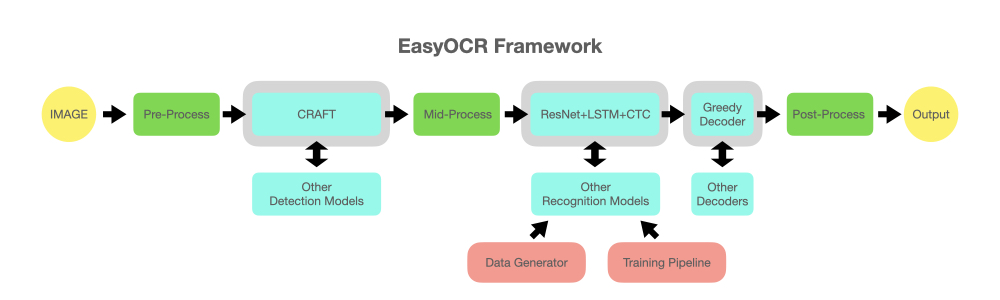
\includegraphics[scale=0.4]{obrazky/easyocr_framework.jpeg}
    \caption{Diagram of EasyOCR pipeline. Grey slots are placeholders for models. The mentioned models are the ones used as default. \cite{easyocr2}}
    \label{img:easyocrPipeline}
\end{figure}

\subsection{Keras-ocr}

keras-ocr is a python library used for detecting and recognizing text in images created by Fausto Morales. It works with variety of languages and with different writing scripts. It allows computing on CPU as well as on GPU.  It unites the CRAFT text detection model and an implementation in Keras python library of CRNN for recognizing text, worth mentioning this is a different implementation of CRNN than in EasyOCR.\cite{keras-ocr1}

On the official website\footnote{\url{https://pypi.org/project/keras-ocr/}} of the package there is a comparison of this method with two other OCR APIs -- Google Cloud Vision and AWS Rekognition. Their performance was tested on 1,000 images from the COCO-Text validation set using a basic pretrained model of each method. None of the investigated methods Michalovice, 293 01 Mlada Boleslavperformed poorly; however, AWS Rekognition had the worst precision and recall results. Google's method and keras-ocr has similar results. It is important to mention that no tuning parameters were used in any of these methods. Another candidate for comparison was Tesseract but it performed on very badly on given data, most likely due to the fact that Tesseract is suitable for scanned documents rather than for photos of real life scenery and objects with text. \cite{keras-ocr1}

CRAFT already provides a pretrained model which can be used directly without modification for text detection or it is used as initial model for training a new model on new data. This model was trained on three datasets (SynthText, IC13, IC17) and supports English and multi language text detection. \cite{craft1}
Similarly for recognition, CRNN also has a pretrained model  This model was trained on the synthetic word dataset which consists of 9 million images with vocabulary of 90K English words. \cite{synth}
To use these models in the keras-ocr library one either doesn't specify anything and use the defaults, or pass the value \texttt{clovaai-general} for the CRAFT pretrained model or \texttt{kurapan} for the CRNN model.

Keras-ocr offers preprocessing for four public datasets though any text image dataset can be examined using this tool. These four datasets are: BornDigital dataset, COCO-Text dataset, ICDAR 2013 dataset, ICDAR 2019 dataset (only Latin-only scripts).\cite{keras-ocrDocu}

\subsection{AWS Rekognition}

\subsection{Google Cloud Vision}

Google Cloud Vision is software from Google which consist of two products: AutoML Vision and Vision API. Vision API detects objects, faces and text from images with already pretrained model. With AutoML Vision user can train custom model from own data. It has free and paid version with a GUI. 

API for python